% When dense optical flow stops reporting the hand.
%
% No artifact number is typed in this file. Each one is a macro (\cg...) defined in
% generated/numbers.tex by scripts/export_paper_tables.py from the committed results, and every
% table and figure is a generated file. tests/test_paper.py fails on a stale generated file, on
% a bare number in the prose that is not on its short allowlist, and on a PDF whose extracted
% text has lost a citation or a number (vernier's paper once lost an abstract to doubled
% backslashes while the build stayed green).
\documentclass[11pt]{article}

\usepackage[margin=1.1in]{geometry}
\usepackage{booktabs}
\usepackage{graphicx}
\usepackage{tikz}
\usepackage{pgfplots}
\usetikzlibrary{calc}
\usepgfplotslibrary{fillbetween}
\pgfplotsset{compat=1.18}
\usepackage{amsmath}
\usepackage{microtype}
\usepackage{url}
\usepackage[hidelinks]{hyperref}
\usepackage[numbers,sort&compress]{natbib}

\setlength{\tabcolsep}{4pt}
\sloppy

% generated by scripts/export_paper_tables.py; do not edit
\newcommand{\cgAmendments}{5}
\newcommand{\cgArxivA}{0}
\newcommand{\cgAssumedMedian}{612.4}
\newcommand{\cgBelowNinety}{7}
\newcommand{\cgBgDist}{2.5}
\newcommand{\cgBudgetMmS}{26.7}
\newcommand{\cgBudgetPct}{4.4}
\newcommand{\cgBudgetPctHi}{5.7}
\newcommand{\cgBudgetPctLo}{4.6}
\newcommand{\cgCardClaims}{12}
\newcommand{\cgCardUntested}{7}
\newcommand{\cgCardVerdict}{NOT\_VERIFIED}
\newcommand{\cgCorpusFactories}{85}
\newcommand{\cgCorpusHours}{10{,}000}
\newcommand{\cgDispAfter}{34.2}
\newcommand{\cgDispKnee}{22.8}
\newcommand{\cgDispLow}{5.7}
\newcommand{\cgDutyPricing}{68}
\newcommand{\cgFreezeShort}{e459aa3}
\newcommand{\cgGainAfterMax}{0.42}
\newcommand{\cgGainAfterMean}{0.25}
\newcommand{\cgGainAfterMin}{0.14}
\newcommand{\cgGainAfterPub}{0.20}
\newcommand{\cgGainAtKneeMax}{0.99}
\newcommand{\cgGainAtKneeMean}{0.88}
\newcommand{\cgGainAtKneeMin}{0.58}
\newcommand{\cgGainAtKneePub}{0.99}
\newcommand{\cgGainAtKneeSd}{0.14}
\newcommand{\cgHalBound}{0.25}
\newcommand{\cgHalLossLargeHi}{6.6}
\newcommand{\cgHalLossLargeLo}{0.0}
\newcommand{\cgHalLossLargeMid}{2.6}
\newcommand{\cgHalLossMeanHi}{6.0}
\newcommand{\cgHalLossMeanLo}{0.0}
\newcommand{\cgHalLossMeanMid}{0.7}
\newcommand{\cgHalLossSmallHi}{4.5}
\newcommand{\cgHalLossSmallLo}{0.0}
\newcommand{\cgHalLossSmallMid}{0.0}
\newcommand{\cgHalTrueHi}{6.9}
\newcommand{\cgHalTrueLo}{1.6}
\newcommand{\cgHalTrueMid}{4.7}
\newcommand{\cgHalfAngle}{67.9}
\newcommand{\cgHalfFarMax}{32.4}
\newcommand{\cgHalfFarMin}{26.1}
\newcommand{\cgHalfFineMax}{32.6}
\newcommand{\cgHalfFineMean}{28.2}
\newcommand{\cgHalfFineMin}{23.6}
\newcommand{\cgHalfFineN}{20}
\newcommand{\cgHalfFineSd}{2.7}
\newcommand{\cgHalfRaftMax}{43.2}
\newcommand{\cgHalfRaftMean}{40.4}
\newcommand{\cgHalfRaftMin}{37.4}
\newcommand{\cgHalfRaftSd}{1.8}
\newcommand{\cgHandBreadth}{85}
\newcommand{\cgHandDist}{0.45}
\newcommand{\cgKneeFineMax}{27.3}
\newcommand{\cgKneeFineMean}{24.8}
\newcommand{\cgKneeFineMin}{22.8}
\newcommand{\cgKneeFineN}{13}
\newcommand{\cgKneeFineSd}{1.6}
\newcommand{\cgLensChecked}{16}
\newcommand{\cgLensShipped}{2{,}144}
\newcommand{\cgMmPerPx}{0.88}
\newcommand{\cgNSeeds}{20}
\newcommand{\cgNSeedsRaft}{11}
\newcommand{\cgPairInterval}{33}
\newcommand{\cgPreregVersion}{1.5.0}
\newcommand{\cgPubSeed}{11}
\newcommand{\cgPublishedRows}{72}
\newcommand{\cgPubmedA}{0}
\newcommand{\cgPubmedB}{1}
\newcommand{\cgPubmedC}{7}
\newcommand{\cgPxAtMedian}{23}
\newcommand{\cgRaftAfterMean}{0.80}
\newcommand{\cgRaftDevGap}{0.0002}
\newcommand{\cgRaftGainSmallMean}{0.98}
\newcommand{\cgRaftGainSmallSd}{0.03}
\newcommand{\cgRaftSmall}{0.30}
\newcommand{\cgRaftSmallPx}{2.8}
\newcommand{\cgRatio}{0.18}
\newcommand{\cgRepoCreated}{8 September 2026}
\newcommand{\cgResFarneback}{1.22}
\newcommand{\cgResGeom}{1.15}
\newcommand{\cgResRaft}{1.01}
\newcommand{\cgRotBudget}{26.5}
\newcommand{\cgRotFisheye}{10.1}
\newcommand{\cgRotNarrow}{0.13}
\newcommand{\cgRotRatio}{76}
\newcommand{\cgSeedMeasurements}{1{,}039}
\newcommand{\cgShelfMax}{0.21}
\newcommand{\cgShelfMean}{0.19}
\newcommand{\cgShelfMin}{0.17}
\newcommand{\cgShelfRaftMean}{0.18}
\newcommand{\cgShelfRaftSd}{0.00}
\newcommand{\cgShelfSd}{0.01}
\newcommand{\cgSibLabels}{153}
\newcommand{\cgSibOver}{10}
\newcommand{\cgSibOverOf}{33}
\newcommand{\cgSibUnder}{2}
\newcommand{\cgSibUnderOf}{120}
\newcommand{\cgSpeedAfter}{903}
\newcommand{\cgSpeedAtKnee}{602}
\newcommand{\cgSpeedHi}{1288.0}
\newcommand{\cgSpeedLo}{255.3}
\newcommand{\cgSpeedRowHi}{903}
\newcommand{\cgSpeedRowLo}{301}
\newcommand{\cgSpeedRowMid}{602}
\newcommand{\cgTransBudgetCm}{3.1}
\newcommand{\cgTransFloorFive}{43.6}
\newcommand{\cgVendorFrames}{10{,}000}
\newcommand{\cgVendorPct}{91.66}
\newcommand{\cgVendorPctEgo}{50.07}
\newcommand{\cgVendorPctEpic}{85.04}
\newcommand{\cgWidthGainA}{0.81}
\newcommand{\cgWidthGainB}{0.88}
\newcommand{\cgWidthGainC}{0.32}
\newcommand{\cgWidthGainD}{0.22}
\newcommand{\cgWidthGainMaxA}{0.97}
\newcommand{\cgWidthGainMaxB}{0.99}
\newcommand{\cgWidthGainMaxC}{0.60}
\newcommand{\cgWidthGainMaxD}{0.31}
\newcommand{\cgWidthGainMinA}{0.50}
\newcommand{\cgWidthGainMinB}{0.58}
\newcommand{\cgWidthGainMinC}{0.17}
\newcommand{\cgWidthGainMinD}{0.18}
\newcommand{\cgWidthHalfA}{17.6}
\newcommand{\cgWidthHalfB}{29.4}
\newcommand{\cgWidthHalfC}{30.3}
\newcommand{\cgWidthHalfD}{37.3}
\newcommand{\cgWidthHalfMmSA}{927}
\newcommand{\cgWidthHalfMmSB}{778}
\newcommand{\cgWidthHalfMmSC}{533}
\newcommand{\cgWidthHalfMmSD}{493}
\newcommand{\cgWidthHalfSdA}{4.3}
\newcommand{\cgWidthHalfSdB}{1.6}
\newcommand{\cgWidthHalfSdC}{3.5}
\newcommand{\cgWidthHalfSdD}{0.6}
\newcommand{\cgWidthSpeedA}{602}
\newcommand{\cgWidthSpeedB}{602}
\newcommand{\cgWidthSpeedC}{602}
\newcommand{\cgWidthSpeedD}{602}


\title{When Dense Optical Flow Stops Reporting the Hand:\\
An Instrument Check for Reading Egocentric Factory Video\\ as Hand Activity Level}
\author{Caio Theodoro\\ \small Independent}
\date{23 November 2026}

\begin{document}
\maketitle

\begin{abstract}
\noindent
Build AI publishes that \cgVendorPct{}\% of \cgVendorFrames{} sampled frames of its Egocentric-10K
factory corpus show the camera wearer actively manipulating an object, as labelled by a
vision-language model. A share of time spent working with the hands is a duty cycle, and duty
cycle is one of the two inputs to the ACGIH Hand Activity Level (HAL). I pre-registered a
measurement of the corpus as HAL before writing code. It has not run, because of cost, and no
ergonomist has scored anything. So this note makes no claim about the corpus, about the vendor's
figure, or about whether the instrument is accurate. It reports the one check that needs no
corpus: whether dense optical flow inside a hand box reports hand speed, tested on rendered
scenes under the corpus's published fisheye lens, with a moving camera over a static hand
plane, where the true flow is known. Over
\cgNSeeds{} texture seeds, the ratio of recovered to true flow stays near one up to about
\cgDispKnee{} px of hand motion between the two frames, falls through one half at \cgWidthHalfB{} px on a nine-point grid, and settles at \cgShelfMean{} (sd \cgShelfSd{}), the ratio of the two assumed
scene depths (\cgRatio{}): in this scene, past the crossing the estimator reports the background. RAFT-small
crosses later, at \cgHalfRaftMean{} px over \cgNSeedsRaft{} seeds, and lands on the same shelf. At
the corpus median speed the pre-registration assumes, and the clip's own frame interval, the
hand moves \cgPxAtMedian{} px. That is the edge of the transition, where mean gain is
\cgGainAtKneeMean{} (range \cgGainAtKneeMin{} to \cgGainAtKneeMax{}) against an error budget of
\cgBudgetPct{}\% of speed. The location of the crossing belongs to this scene and may not transfer: the scene is
one geometry with no occlusion, blur or noise, two estimators were tried at their defaults, and
the registered pair spacing was changed after this check failed. Three claims in an essay I published earlier \citep{theodoro2026essay} from a single seed did not
survive the seeds, and are corrected here. Not peer reviewed.
\end{abstract}

\section{What this note does not show}
\label{sec:notshow}

The measurement the project exists to make has not run. It is a reading of a \cgCorpusHours{}-hour
factory corpus as HAL, and its cost is stated in the repository's cost ledger as blocked on money and
on one licence acceptance. Nothing below is a result about that corpus.

No ergonomist, certified or otherwise, has scored a clip, so there is no agreement statistic of
any kind. The instrument is unvalidated against professional assessment, and nothing in this
note narrows that gap. Peak force cannot be read from video, so the full ACGIH threshold limit
value is never computed. Only its HAL axis is in scope, and every record the project writes
says so.

The vendor's number is a share of sampled frames that a language model called manipulation. It is
not a duty cycle of any worker or any job, and Section~\ref{sec:viewpoint} says what has to be
true before it could stand in for one. I do not compute HAL from it anywhere in this note.

What I did run is a check on one input to the instrument, hand speed from dense optical flow, on
rendered frames. It is a small result with a stated scope. It is also the only part of the
project a stranger can reproduce with no corpus access, no token and no GPU.

\section{The viewpoint}
\label{sec:viewpoint}

\paragraph{Hand Activity Level.}
The ACGIH threshold limit value for HAL rates repetitive hand work from 0 to 10, from how often
the hands exert and what share of the cycle they spend exerting \citep{latko1997,radwin2015}.
Two published equations, both regression fits to the ACGIH 2001 look-up table, turn the inputs
into a rating: one from exertion frequency and duty cycle \citep{radwin2015}, one from RMS hand
speed and duty cycle \citep{akkas2015}. The second is
\begin{equation}
\mathrm{HAL} = 10\,\sigma\!\left(-15.87 + 0.02\,D + 2.25\ln S\right),
\end{equation}
with $\sigma$ the logistic function, $D$ the duty cycle in percent and $S$ the RMS hand speed in
mm/s. It was fitted on speeds from \cgSpeedLo{} to \cgSpeedHi{} mm/s. The scale is not
decorative: HAL combined with peak force is associated with carpal tunnel syndrome incidence in a pooled cohort \citep{kapellusch2014}.

\paragraph{The vendor's figure.}
Build AI sells egocentric video recorded in factories. The evaluation release's dataset card
publishes quality figures for it \citep{buildai2025eval}. It states that the authors
``randomly sample 10k frames from each dataset and run them through a gemini-2.5-flash'', and
defines active manipulation as the wearer ``visibly using their hands to work on, modify,
assemble, process, or handle physical objects, materials, components in pursuit of a specific
goal''. The model is told to answer ``no'' when the action is ambiguous. The published figure
for Egocentric-10K is \cgVendorPct{}\%, against \cgVendorPctEgo{}\% for Ego4D
\citep{grauman2022ego4d} and \cgVendorPctEpic{}\% for EPIC-KITCHENS-100 \citep{damen2022epic100}.
The corpus is \cgCorpusHours{} hours across \cgCorpusFactories{} factories
\citep{buildai2025corpus}. The card carries no interval and no human label. Every statement in
this paragraph is copied from the vendor's pages on the date I retrieved them, and the copy is
\texttt{results/vendor\_claim.json}.

\paragraph{Why the two meet.}
The fraction of sampled instants in a state is, if the instants are drawn uniformly over time,
the fraction of time in that state. That is a duty cycle. The TLV's own definition of an
exertion is the hand holding, manipulating, triggering, pushing, pulling or otherwise handling an
object, which is close to what the vendor's prompt asks a model to find \citep{radwin2015}.

That is an analogy, and three things make it weaker than it sounds. The vendor's figure pools
every worker, task and idle minute in the sample, so it is a corpus prevalence, and the TLV's
duty cycle belongs to a job. The card does not say the frames were drawn uniformly over time.
And the label is a model's, once: in a sibling audit of the same figures, I found that the same
kind of judge over-called manipulation on \cgSibOver{} of \cgSibOverOf{} frames where over-calling
was possible against \cgSibUnder{} of \cgSibUnderOf{} for under-calling, on a \cgSibLabels{}-frame set
labelled by one rater \citep{theodoro2026vernier}.
In that audit the
judge's errors ran mostly one way, so a share from that kind of label is more likely too high than
too low. That is a statement about the kind of label, not a measurement of the vendor's figure.
So the reading that survives is narrower: the same label, taken per clip and not pooled, would be
the duty-cycle input, and a hand-speed estimate for the same clip would be the other. Whether the
label can express the TLV's exertion is the sharpest open objection in the repository's own list
of objections to itself, which marks it fatal if it fails.

\paragraph{Why nobody has read it that way.}
Automated ergonomic assessment from video is mature, and HAL itself has been recovered from
video since 2013 by one group, and the work I could open used a fixed camera
\citep{chen2013,akkas2016,radwin2023,lin2026hal}. I read the two equation papers in full and these
only as abstracts. The whole-body indices RULA and REBA are
the usual targets of the general systems \citep{agostinelli2024,massiris2022ergoexplorer,yazdani2022dula},
and they score trunk, neck and legs, which a head-mounted camera does not see. The hand-and-wrist
standards are not ill-posed from that viewpoint, and I found nothing that applies one to
egocentric video. The nearest work measures the share of time hands interact with objects, with
a head-worn camera, to track hand use after spinal cord injury; it does not mention
occupational exposure \citep{likitlersuang2019}.

The gate that asked this was run on 5 September 2026 and cleared narrowly. I reran its three
PubMed queries on 23 November 2026. They returned \cgPubmedA{}, \cgPubmedB{} and \cgPubmedC{}
hits, the same counts as in September; the one hit for the second query is a surface-EMG paper
that is not video. An arXiv title-and-abstract query for the phrase ``hand activity level''
returned \cgArxivA{}. That is a search result, not a proof of absence, and the record is
\texttt{results/provenance.json}.

\section{What was fixed before any result}
\label{sec:prereg}

Pre-registration binds an analysis plan before outcomes are known \citep{nosek2018}. Here it
fixed the following, in \texttt{docs/PRE-REGISTRATION.md}, before a line of the pipeline's source
existed.

The corpus is the raw release at one pinned revision, because the evaluation release's frame
identifiers carry no clip, worker or factory. Frames are read at 4 Hz. HAL is computed only by
the two published equations above, and never by an approximation of mine. The speed path is
primary and a spectral bout frequency is the cross-check. Intervals cluster over factory and
worker together, since clips from one worker share task, station and shift. The reporting unit is
the corpus, plus factory-size terciles that clear a k-anonymity floor of five factories and fifty
workers with no factory above 40\% of a stratum; no worker and no factory is ever a reporting unit,
because the measured object is people at work. Peak force is never imputed. The speed path's
residual floor (the apparent speed a static hand produces under camera motion alone, Section~\ref{sec:check}) under the corpus's own lens must be at most \cgHalBound{} HAL at the corpus median
speed. Five hypotheses (H1 to H5, which the card splits into sub-claims) carry numeric bounds and the condition that falsifies each; a negative
control on two other egocentric corpora is meant to show the pipeline responds to repetitive work
and not to hands or head motion. The main draw has two arms, 40{,}000 clips or 200, and which
arm runs is decided by one pilot result.

Two things limit what that buys. The freeze is a git commit (\cgFreezeShort{}); every commit that
adds a source file descends from it, and \texttt{scripts/validate.py} checks that by ancestry and
not by timestamp. But the repository became public on \cgRepoCreated{}, after the one-factory
pilot had run, and the freeze has no signed tag, no registry entry and no third-party timestamp.
A reader has the author's history and nothing else. The deposit of this note is a deposit of a
paper; it does not date the registration. And pre-registration bounds analytic flexibility, not
the choice of what to register.

The file was amended \cgAmendments{} times, to version \cgPreregVersion{}, each time through a
dated decision with a reversal clause and a quotation of the sentence replaced. The last
amendment matters to this note. The speed pair had been read as two frames $1/4$ s apart (the 4 Hz analysis rate taken as the pair spacing). The
synthetic sweep below showed that at that spacing both estimators report the background across
the fitted speed range, and the sentence was amended to mean the clip's own frame interval,
about \cgPairInterval{} ms. No real speed had been measured, so the amendment predates any
outcome; it did not predate the instrument check, and a reader should weigh it as a change made
because the check failed.

A pilot on one factory has run end to end. Its values are never published, because a single
factory can be named; only verdicts are. Table~\ref{tab:card} is the measurement card as
committed. Its sources sit with the withheld pilot values, so a reader cannot check any row from
the repository, and nothing in this note rests on one. Of the \cgCardClaims{} claims, \cgCardUntested{} are untested.
One failure is worth stating: the spectral frequency path disagreed with transition counting by far
more than its registered bound, and the obvious repair was left unapplied because the result had
already been seen.

\begin{table}[t]
\centering\small
\begin{tabular}{@{}llp{9.2cm}@{}}
\toprule
Claim & status & statement \\
\midrule
H1 & untested & duty cycle is a property of the clip, not of the labeller \\
H1a & untested & duty cycle agrees across label sources \\
H1b & holds & duty cycle agrees across sampling rates \\
H2 & failed & exertion frequency is recoverable without segmenting exertions \\
H2a & failed & spectral and transition-counting frequency agree \\
H2b & holds & enough clips carry a resolvable dominant cycle \\
H2c & holds & detector coverage and flow-null rate clear their bounds \\
H3 & untested & the corpus median HAL is plausible against the pooled cohort \\
H4 & untested & exposure structure is between sites, not between people \\
H5 & untested & clip observations are not independent \\
NC-dc & untested & the pipeline separates factory work from non-factory work on duty cycle \\
NC-f & untested & the pipeline separates factory work from kitchen work on the speed path \\
\bottomrule
\end{tabular}

\caption{The pre-registered claims and their recorded status, from
\texttt{MEASUREMENT\_CARD.json}. The card's verdict is \cgCardVerdict{}. Pilot rows come from one
factory whose values are withheld.}
\label{tab:card}
\end{table}

\section{The instrument check}
\label{sec:check}

\paragraph{Design.}
Hand speed in the pipeline is the RMS of residual optical flow inside a detected hand box, with
ego-motion estimated as the median flow over the complement of the box and subtracted, and the
result scaled to mm/s by the box width against an \cgHandBreadth{} mm hand breadth. Before any
real frame touched it, I asked what that rule does on frames where the answer is known.

The scene is two fronto-parallel textured planes seen through the corpus's published fisheye
lens (Kannala--Brandt, \cgHalfAngle{} degrees of half-angle) \citep{kannala2006}: a hand plane at
\cgHandDist{} m and a background at \cgBgDist{} m. Both distances are stated assumptions about a
workstation, and the shelf moves with them. The camera translates sideways
between the two frames, which gives the static hand its motion relative to the camera and the
background its own, in the ratio of the depths. The true flow is analytic. The quantity is
\emph{gain}: the median recovered flow magnitude inside the hand box over the median true
magnitude there. A gain of one recovers the motion; a gain of \cgRatio{} reports under a fifth
of it. The two estimators are OpenCV's Farneback \citep{farneback2003} at its default pyramid and
window, and torchvision's RAFT-small with its default weights \citep{teed2020raft}, run on a CPU.
The seed changes only the texture. The pair interval is \cgPairInterval{} ms, and it only
rescales displacement into mm/s.

\paragraph{The seed spread.}
The published curve was one seed, number \cgPubSeed{}. I repeated the sweep over \cgNSeeds{} seeds for
Farneback and \cgNSeedsRaft{} for RAFT-small, because a single run is not an interval. The spread
is the texture's and nothing else; it says nothing about factory video.

\begin{figure}[t]
\centering
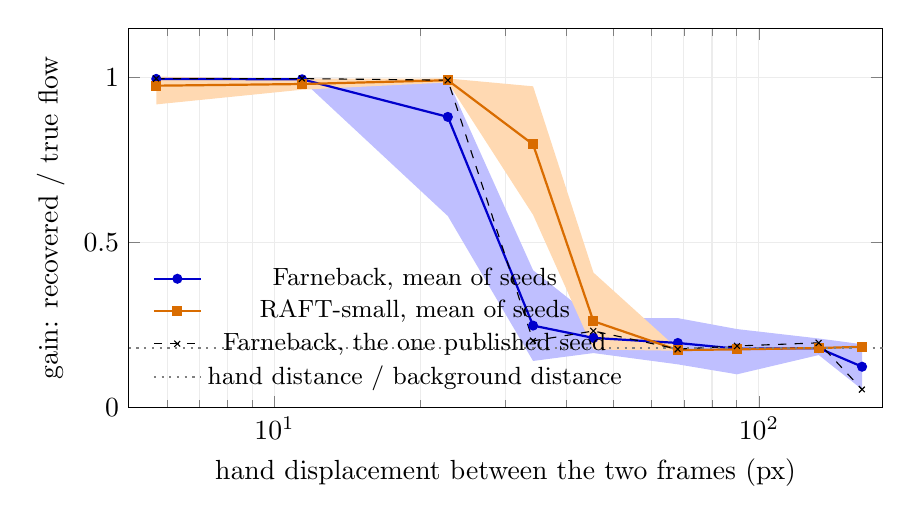
\begin{tikzpicture}
\begin{axis}[width=0.92\linewidth,height=6.4cm,xmode=log,xlabel={hand displacement between the two frames (px)},ylabel={gain: recovered / true flow},ymin=0,ymax=1.15,xmin=5,xmax=180,legend style={at={(0.02,0.02)},anchor=south west,font=\small,draw=none,fill=none},grid=both,grid style={gray!15}]
\addplot[name path=fl,draw=none,forget plot] coordinates {(5.7,0.9954) (11.399,0.9921) (22.794,0.5807) (34.181,0.1415) (45.539,0.1654) (68.025,0.1312) (90.136,0.101) (132.883,0.1594) (163.312,0.0552)};
\addplot[name path=fh,draw=none,forget plot] coordinates {(5.7,0.9975) (11.399,0.9973) (22.794,0.9925) (34.181,0.4165) (45.539,0.2711) (68.025,0.2713) (90.136,0.2381) (132.883,0.2096) (163.312,0.1921)};
\addplot[blue!25,forget plot] fill between[of=fl and fh];
\addplot[name path=rl,draw=none,forget plot] coordinates {(5.7,0.9191) (11.399,0.9637) (22.794,0.9856) (34.181,0.5843) (45.539,0.1763) (68.025,0.1724) (90.136,0.1758) (132.883,0.1801) (163.312,0.1839)};
\addplot[name path=rh,draw=none,forget plot] coordinates {(5.7,1.0034) (11.399,0.997) (22.794,0.9977) (34.181,0.9739) (45.539,0.4094) (68.025,0.1779) (90.136,0.1769) (132.883,0.181) (163.312,0.1849)};
\addplot[orange!30,forget plot] fill between[of=rl and rh];
\addplot[blue!80!black,thick,mark=*,mark size=1.4pt] coordinates {(5.7,0.9964) (11.399,0.9952) (22.794,0.8812) (34.181,0.2487) (45.539,0.2113) (68.025,0.196) (90.136,0.1785) (132.883,0.1804) (163.312,0.124)};
\addlegendentry{Farneback, mean of seeds}
\addplot[orange!85!black,thick,mark=square*,mark size=1.4pt] coordinates {(5.7,0.9758) (11.399,0.9809) (22.794,0.9923) (34.181,0.7978) (45.539,0.2619) (68.025,0.1745) (90.136,0.1766) (132.883,0.1807) (163.312,0.1844)};
\addlegendentry{RAFT-small, mean of seeds}
\addplot[black,dashed,thin,mark=x,mark size=1.6pt] coordinates {(5.7,0.9973) (11.399,0.9973) (22.794,0.9925) (34.181,0.2024) (45.539,0.2323) (68.025,0.1773) (90.136,0.1869) (132.883,0.1964) (163.312,0.0552)};
\addlegendentry{Farneback, the one published seed}
\addplot[gray,dotted,thick] coordinates {(5,0.18)(180,0.18)};
\addlegendentry{hand distance / background distance}
\end{axis}
\end{tikzpicture}

\caption{Gain against hand displacement at 960$\times$540. Lines are the mean over seeds; bands
are the minimum and maximum. The dashed line is the one seed I published earlier (seed number \cgPubSeed{}). It reads at the top of the band at \cgDispKnee{} px and below the mean at \cgDispAfter{} px, so it shows a sharper drop than the average texture does.}
\label{fig:gain}
\end{figure}

Figure~\ref{fig:gain} and Table~\ref{tab:gain} give the result. Below about \cgDispKnee{} px
Farneback recovers the hand's motion. The mean gain at \cgDispKnee{} px is \cgGainAtKneeMean{}
(sd \cgGainAtKneeSd{}, range \cgGainAtKneeMin{} to \cgGainAtKneeMax{}), and the published seed read
\cgGainAtKneePub{} there. At \cgDispAfter{} px the mean is \cgGainAfterMean{}, with a range of
\cgGainAfterMin{} to \cgGainAfterMax{}, and the published seed read \cgGainAfterPub{}. So the
single-seed curve showed a cliff between two grid points, and the seeds show a transition whose
location depends on the texture. On a finer grid across it, gain crosses one half at
\cgHalfFineMean{} px (sd \cgHalfFineSd{}, range \cgHalfFineMin{} to \cgHalfFineMax{}, all
\cgHalfFineN{} seeds), and \cgBelowNinety{} of \cgNSeeds{} seeds are already below 0.9 at
\cgDispKnee{} px.

\begin{table}[t]
\centering\small
\begin{tabular}{@{}rrrcrrc@{}}
\toprule
 & \multicolumn{3}{c}{Farneback} & \multicolumn{3}{c}{RAFT-small} \\
\cmidrule(lr){2-4}\cmidrule(lr){5-7}
Displacement (px) & mean & sd & range & mean & sd & range \\
\midrule
5.7 & 1.00 & 0.00 & 1.00--1.00 & 0.98 & 0.03 & 0.92--1.00 \\
11.4 & 1.00 & 0.00 & 0.99--1.00 & 0.98 & 0.01 & 0.96--1.00 \\
22.8 & 0.88 & 0.14 & 0.58--0.99 & 0.99 & 0.00 & 0.99--1.00 \\
34.2 & 0.25 & 0.08 & 0.14--0.42 & 0.80 & 0.13 & 0.58--0.97 \\
45.5 & 0.21 & 0.03 & 0.17--0.27 & 0.26 & 0.09 & 0.18--0.41 \\
68.0 & 0.20 & 0.03 & 0.13--0.27 & 0.17 & 0.00 & 0.17--0.18 \\
90.1 & 0.18 & 0.03 & 0.10--0.24 & 0.18 & 0.00 & 0.18--0.18 \\
132.9 & 0.18 & 0.01 & 0.16--0.21 & 0.18 & 0.00 & 0.18--0.18 \\
163.3 & 0.12 & 0.05 & 0.06--0.19 & 0.18 & 0.00 & 0.18--0.18 \\
\bottomrule
\end{tabular}

\caption{Gain by displacement at 960$\times$540, over \cgNSeeds{} seeds for Farneback and
\cgNSeedsRaft{} for RAFT-small. Range is minimum to maximum.}
\label{tab:gain}
\end{table}

\begin{figure}[t]
\centering
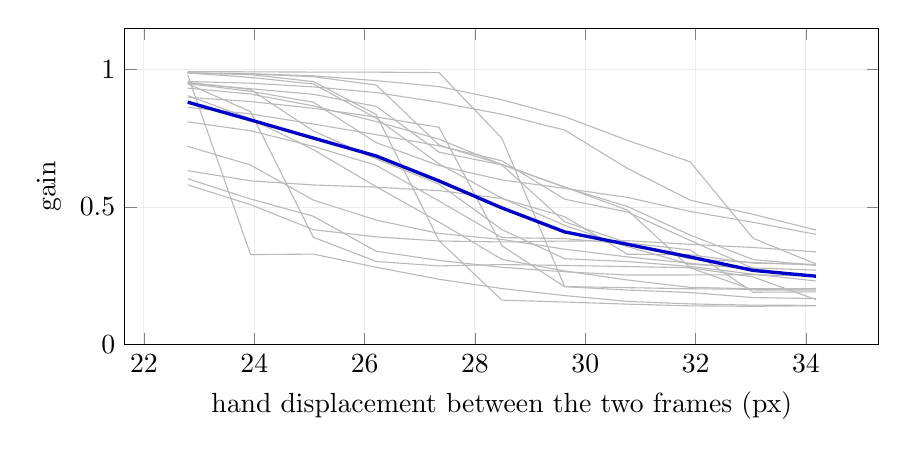
\begin{tikzpicture}
\begin{axis}[width=0.92\linewidth,height=5.6cm,xlabel={hand displacement between the two frames (px)},ylabel={gain},ymin=0,ymax=1.15,grid=both,grid style={gray!15}]
\addplot[gray!55,thin] coordinates {(22.794,0.8987) (23.933,0.8836) (25.071,0.8591) (26.211,0.8274) (27.349,0.7901) (28.488,0.3595) (29.627,0.2105) (30.766,0.1984) (31.904,0.1894) (33.042,0.171) (34.181,0.1674)};
\addplot[gray!55,thin] coordinates {(22.794,0.949) (23.933,0.9206) (25.071,0.8811) (26.211,0.7341) (27.349,0.6505) (28.488,0.5987) (29.627,0.568) (30.766,0.5351) (31.904,0.4837) (33.042,0.4448) (34.181,0.4008)};
\addplot[gray!55,thin] coordinates {(22.794,0.9876) (23.933,0.9837) (25.071,0.9738) (26.211,0.9434) (27.349,0.7258) (28.488,0.6547) (29.627,0.5719) (30.766,0.5018) (31.904,0.398) (33.042,0.3092) (34.181,0.2883)};
\addplot[gray!55,thin] coordinates {(22.794,0.988) (23.933,0.9847) (25.071,0.977) (26.211,0.9595) (27.349,0.9379) (28.488,0.8901) (29.627,0.8287) (30.766,0.7424) (31.904,0.6642) (33.042,0.3867) (34.181,0.2932)};
\addplot[gray!55,thin] coordinates {(22.794,0.9863) (23.933,0.9815) (25.071,0.956) (26.211,0.8364) (27.349,0.378) (28.488,0.1618) (29.627,0.155) (30.766,0.1472) (31.904,0.1409) (33.042,0.1393) (34.181,0.1415)};
\addplot[gray!55,thin] coordinates {(22.794,0.5807) (23.933,0.5087) (25.071,0.4177) (26.211,0.3917) (27.349,0.3767) (28.488,0.3733) (29.627,0.3764) (30.766,0.3779) (31.904,0.3646) (33.042,0.3531) (34.181,0.3372)};
\addplot[gray!55,thin] coordinates {(22.794,0.9507) (23.933,0.93) (25.071,0.9098) (26.211,0.8661) (27.349,0.6996) (28.488,0.6532) (29.627,0.4464) (30.766,0.3701) (31.904,0.3441) (33.042,0.1904) (34.181,0.1918)};
\addplot[gray!55,thin] coordinates {(22.794,0.7206) (23.933,0.6528) (25.071,0.5254) (26.211,0.4528) (27.349,0.4041) (28.488,0.3823) (29.627,0.3469) (30.766,0.3188) (31.904,0.2956) (33.042,0.2734) (34.181,0.2483)};
\addplot[gray!55,thin] coordinates {(22.794,0.6323) (23.933,0.5952) (25.071,0.5804) (26.211,0.5723) (27.349,0.5597) (28.488,0.531) (29.627,0.4652) (30.766,0.3286) (31.904,0.3269) (33.042,0.2961) (34.181,0.2916)};
\addplot[gray!55,thin] coordinates {(22.794,0.8094) (23.933,0.7773) (25.071,0.7207) (26.211,0.6515) (27.349,0.5222) (28.488,0.3891) (29.627,0.3854) (30.766,0.3657) (31.904,0.3119) (33.042,0.2987) (34.181,0.289)};
\addplot[gray!55,thin] coordinates {(22.794,0.9323) (23.933,0.9108) (25.071,0.8677) (26.211,0.8106) (27.349,0.7468) (28.488,0.6542) (29.627,0.5728) (30.766,0.4889) (31.904,0.279) (33.042,0.1988) (34.181,0.1983)};
\addplot[gray!55,thin] coordinates {(22.794,0.9925) (23.933,0.9915) (25.071,0.9906) (26.211,0.9903) (27.349,0.9886) (28.488,0.7502) (29.627,0.2111) (30.766,0.2071) (31.904,0.2031) (33.042,0.2011) (34.181,0.2024)};
\addplot[gray!55,thin] coordinates {(22.794,0.9564) (23.933,0.9502) (25.071,0.9368) (26.211,0.9162) (27.349,0.8808) (28.488,0.8374) (29.627,0.7797) (30.766,0.6403) (31.904,0.525) (33.042,0.4738) (34.181,0.4165)};
\addplot[gray!55,thin] coordinates {(22.794,0.948) (23.933,0.8468) (25.071,0.3902) (26.211,0.3023) (27.349,0.2862) (28.488,0.2911) (29.627,0.2877) (30.766,0.2838) (31.904,0.2794) (33.042,0.2462) (34.181,0.1637)};
\addplot[gray!55,thin] coordinates {(22.794,0.8625) (23.933,0.8386) (25.071,0.8018) (26.211,0.7632) (27.349,0.7226) (28.488,0.6683) (29.627,0.5286) (30.766,0.4819) (31.904,0.3786) (33.042,0.2771) (34.181,0.2466)};
\addplot[gray!55,thin] coordinates {(22.794,0.9874) (23.933,0.9712) (25.071,0.9474) (26.211,0.8228) (27.349,0.6569) (28.488,0.5325) (29.627,0.4337) (30.766,0.356) (31.904,0.2919) (33.042,0.2789) (34.181,0.2707)};
\addplot[gray!55,thin] coordinates {(22.794,0.9801) (23.933,0.3274) (25.071,0.329) (26.211,0.2813) (27.349,0.2376) (28.488,0.2039) (29.627,0.1783) (30.766,0.1571) (31.904,0.148) (33.042,0.1435) (34.181,0.1427)};
\addplot[gray!55,thin] coordinates {(22.794,0.905) (23.933,0.8211) (25.071,0.7087) (26.211,0.5739) (27.349,0.4457) (28.488,0.3099) (29.627,0.2678) (30.766,0.2349) (31.904,0.2081) (33.042,0.203) (34.181,0.2039)};
\addplot[gray!55,thin] coordinates {(22.794,0.6029) (23.933,0.5293) (25.071,0.4666) (26.211,0.3395) (27.349,0.3062) (28.488,0.2811) (29.627,0.2647) (30.766,0.253) (31.904,0.2533) (33.042,0.2542) (34.181,0.2484)};
\addplot[gray!55,thin] coordinates {(22.794,0.9534) (23.933,0.9272) (25.071,0.7764) (26.211,0.675) (27.349,0.5835) (28.488,0.4182) (29.627,0.3123) (30.766,0.3019) (31.904,0.2843) (33.042,0.2561) (34.181,0.2315)};
\addplot[blue!80!black,very thick] coordinates {(22.794,0.8812) (23.933,0.8166) (25.071,0.7508) (26.211,0.6855) (27.349,0.595) (28.488,0.497) (29.627,0.4096) (30.766,0.3645) (31.904,0.3185) (33.042,0.2698) (34.181,0.2487)};
\end{axis}
\end{tikzpicture}

\caption{Farneback at 960$\times$540 on a fine grid across the transition. One thin line per
seed, mean in blue. The location of the drop moves by several pixels with the texture.}
\label{fig:fine}
\end{figure}

\paragraph{The shelf.}
Past the transition gain does not fall to zero. It sits at \cgShelfMean{} (sd \cgShelfSd{}, range \cgShelfMin{}
to \cgShelfMax{}) for Farneback and at \cgShelfRaftMean{} (sd \cgShelfRaftSd{}) for
RAFT-small, against a depth ratio of \cgRatio{}. At the largest displacement Farneback falls
below the shelf, because it has exceeded its search range and tracks nothing; that second regime
is excluded from the shelf and is not averaged into it. The estimator is no longer measuring the hand.
It has smoothed across the depth discontinuity at the box edge and reports the background, which is further away by that ratio and so moves that much more slowly in pixels. The number it returns is a correct measurement of the wrong object. I infer the mechanism from the gain landing on the ratio; I did not render the flow field to look.

The nine-point-grid crossings are interpolated linearly between points far apart, so for Farneback the fine grid, \cgHalfFineMean{} px, is the better estimate and the nine-point figure, \cgWidthHalfB{} px (sd \cgWidthHalfSdB{}), is for comparing against RAFT-small and across widths.

RAFT-small moves the crossing and leaves the shelf alone. On the same nine-point grid gain
crosses one half at \cgHalfRaftMean{} px (sd \cgHalfRaftSd{}, range \cgHalfRaftMin{} to
\cgHalfRaftMax{}) against \cgWidthHalfB{} for Farneback (range \cgHalfFarMin{} to \cgHalfFarMax{}), and the ranges do not overlap. The crossing belongs to the estimator and the shelf belongs to the geometry. RAFT-small also
under-recovers small motion at the smallest decode: \cgRaftSmall{} at \cgRaftSmallPx{} px at
480$\times$270, one seed.  Two estimators say nothing about a method that models depth. On the shared seed the CPU run
reproduces the published curve, which was measured on a GPU, to within \cgRaftDevGap{}.

\paragraph{Where the corpus's assumed speed sits.}
The pre-registration assumes a corpus median RMS speed of \cgAssumedMedian{} mm/s to price its
error budget. At \cgPairInterval{} ms and \cgMmPerPx{} mm per pixel at 960$\times$540, that speed
moves the hand \cgPxAtMedian{} px (the nearest grid point, \cgDispKnee{} px, is \cgSpeedAtKnee{} mm/s), which is the top edge of the flat part of the curve and the
start of the drop. The registered budget is \cgHalBound{} HAL, which at that speed is
\cgBudgetMmS{} mm/s, or \cgBudgetPct{}\% of the speed (between \cgBudgetPctLo{}\% and
\cgBudgetPctHi{}\% across the band from 400 to 800 mm/s). Mean gain at the matching grid point
is \cgGainAtKneeMean{}. Gain is not the pipeline's speed error, because the subtraction step
changes it, but a recovery of \cgGainAtKneeMean{} on average and \cgGainAtKneeMin{} at worst is
not a recovery within a few percent. At \cgSpeedAfter{} mm/s, inside the fitted range of the
equation, the estimator is on the shelf.

\begin{table}[t]
\centering\small
\begin{tabular}{@{}rrrrcr@{}}
\toprule
True speed (mm/s) & Mean gain & HAL, true & HAL, recovered & HAL, seed range & Loss (mean) \\
\midrule
301 & 1.00 & 1.59 & 1.57 & 1.56--1.58 & 0.01 \\
602 & 0.88 & 4.73 & 4.03 & 2.09--4.68 & 0.70 \\
903 & 0.25 & 6.90 & 0.89 & 0.27--2.37 & 6.02 \\
\bottomrule
\end{tabular}

\caption{An illustration, not a measurement: HAL from the equation at a duty cycle of
\cgDutyPricing{}\% when the speed it is given is the true speed scaled by Farneback's mean gain
at that speed, and over the seed range of the gain. The subtraction of ego-motion is ignored,
which would lower the recovered speed further.}
\label{tab:hal}
\end{table}

Table~\ref{tab:hal} turns gain into HAL points at three speeds. It propagates the synthetic gain
through the published equation and nothing else, at a duty cycle I chose to match the repository's
pricing assumption. The loss is \cgHalLossMeanLo{} points at \cgSpeedRowLo{} mm/s,
\cgHalLossMeanMid{} at \cgSpeedRowMid{} mm/s and \cgHalLossMeanHi{} at \cgSpeedRowHi{} mm/s, against a
registered bound of \cgHalBound{}.

\paragraph{Decode resolution.}
The repository chose 960$\times$540 for the flow decode because a single seed showed it beating
both 480$\times$270 and the larger sizes. Table~\ref{tab:width} puts the four widths at the same
physical motion, about \cgWidthSpeedB{} mm/s. The seeds do not support an optimum. At that speed
the mean gain is \cgWidthGainA{} at 480$\times$270 (range \cgWidthGainMinA{} to \cgWidthGainMaxA{})
and \cgWidthGainB{} at 960$\times$540 (range \cgWidthGainMinB{} to \cgWidthGainMaxB{}); the
ranges overlap almost entirely. What the seeds do support is that 1440 and 1920 wide fall at a
lower physical speed, \cgWidthHalfMmSC{} and \cgWidthHalfMmSD{} mm/s at the half crossing against
\cgWidthHalfMmSB{} at 960, because a finer grid spends the same motion on more pixels. The 480$\times$270 row has the highest crossing speed and the lowest crossing in pixels, and I do not explain it. The grid
is coarse above 480, so I make no claim about how the crossing scales with the hand box.

\begin{table}[t]
\centering\small
\resizebox{\linewidth}{!}{\begin{tabular}{@{}lrrcrrr@{}}
\toprule
Decode & mm/px & px moved & gain at about 600 mm/s & crossing (px) & sd (px) & crossing (mm/s) \\
\midrule
480$\times$270 & 1.76 & 11.4 & 0.81 (0.50--0.97) & 17.6 & 4.3 & 927 \\
960$\times$540 & 0.88 & 22.8 & 0.88 (0.58--0.99) & 29.4 & 1.6 & 778 \\
1440$\times$810 & 0.59 & 34.2 & 0.32 (0.17--0.60) & 30.3 & 3.5 & 533 \\
1920$\times$1080 & 0.44 & 45.6 & 0.22 (0.18--0.31) & 37.3 & 0.6 & 493 \\
\bottomrule
\end{tabular}
}
\caption{Farneback at four decode widths over \cgNSeeds{} seeds. Gain is read at the same
physical motion in every row. The crossing is the displacement where gain first falls through one
half, interpolated linearly on the nine-point grid.}
\label{tab:width}
\end{table}

\begin{figure}[t]
\centering
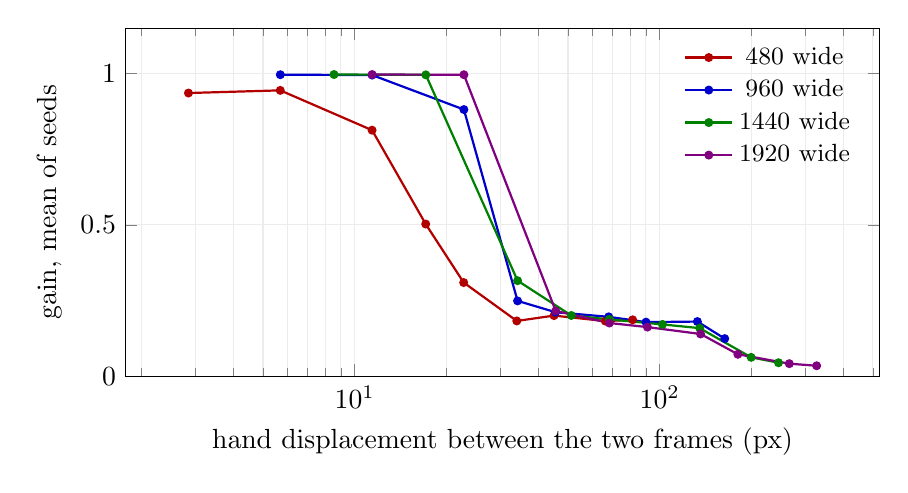
\begin{tikzpicture}
\begin{axis}[width=0.92\linewidth,height=6cm,xmode=log,xlabel={hand displacement between the two frames (px)},ylabel={gain, mean of seeds},ymin=0,ymax=1.15,legend style={at={(0.98,0.98)},anchor=north east,font=\small,draw=none,fill=none},grid=both,grid style={gray!15}]
\addplot[red!70!black,thick,mark=*,mark size=1.2pt] coordinates {(2.849,0.9358) (5.698,0.9446) (11.395,0.813) (17.086,0.5027) (22.759,0.3093) (33.981,0.1824) (45.009,0.2001) (66.327,0.1819) (81.495,0.1862)};
\addlegendentry{480 wide}
\addplot[blue!80!black,thick,mark=*,mark size=1.2pt] coordinates {(5.7,0.9964) (11.399,0.9952) (22.794,0.8812) (34.181,0.2487) (45.539,0.2113) (68.025,0.196) (90.136,0.1785) (132.883,0.1804) (163.312,0.124)};
\addlegendentry{960 wide}
\addplot[green!50!black,thick,mark=*,mark size=1.2pt] coordinates {(8.549,0.997) (17.098,0.9958) (34.191,0.3155) (51.271,0.2005) (68.313,0.1876) (102.058,0.1709) (135.236,0.1586) (199.391,0.0621) (245.091,0.0443)};
\addlegendentry{1440 wide}
\addplot[violet,thick,mark=*,mark size=1.2pt] coordinates {(11.399,0.9969) (22.798,0.9963) (45.588,0.2155) (68.363,0.1756) (91.09,0.1621) (136.1,0.1393) (180.357,0.0722) (265.943,0.0412) (326.912,0.0343)};
\addlegendentry{1920 wide}
\end{axis}
\end{tikzpicture}

\caption{Mean gain against displacement for the four decode widths, over \cgNSeeds{} seeds.}
\label{fig:width}
\end{figure}

\paragraph{Why it hides.}
The pipeline takes ego-motion as the median flow outside the hand box and subtracts it. Past the transition the box already holds the background's flow, so by the rule's own arithmetic the correction removes the signal it was meant to clean and the residual comes out small and ordinary-looking. The sweep does not run the subtraction; this is the rule applied to the measured gain. Every one of the \cgPublishedRows{} rows in the three published sweep files, and every one of the
\cgSeedMeasurements{} seeded measurements (four widths on the nine-point grid, the fine grid, and the
RAFT-small run), returned a finite, non-null field, so no null-rate ceiling and no schema check
has anything to fire on. The residual that a rotation-only synthetic leaves is the one place the
failure shows against a control. Exact geometry leaves \cgResGeom{} px; Farneback leaves
\cgResFarneback{}, above the floor as an estimator's error should be; RAFT-small leaves
\cgResRaft{}, below the floor that exact geometry allows, which is most simply read as recovering less of the field than is there. These are one scene and one seed.

\paragraph{The lens and the subtraction, with no estimator.}
The same subtraction has a second
error that needs no estimator. Rotational flow on a fisheye
varies with radius, and a scalar median over the background cancels a uniform field, not a radial
one. In closed form, a head rotation of 10 degrees per second leaves \cgRotFisheye{} mm/s of
apparent hand speed under the corpus lens and \cgRotNarrow{} mm/s under a narrow one, about
\cgRotRatio{} times more from the same rule. Table~\ref{tab:floor} gives the sweep. The registered
budget is exhausted by \cgRotBudget{} degrees per second of rotation, or \cgTransBudgetCm{} cm/s
of translation, at the assumed median. Whether real head motion sits inside that is unknown until
frames are decoded.

\begin{table}[t]
\centering\small
\begin{tabular}{@{}rrr@{}}
\toprule
Head rotation (deg/s) & corpus fisheye (mm/s) & narrow lens (mm/s) \\
\midrule
2 & 2.02 & 0.03 \\
10 & 10.09 & 0.13 \\
30 & 30.27 & 0.40 \\
60 & 60.50 & 0.81 \\
\bottomrule
\end{tabular}

\caption{Apparent hand speed that a perfectly static hand produces after the ego-motion
subtraction, in exact geometry with no estimator, from \texttt{a14\_translation\_floor.json}.}
\label{tab:floor}
\end{table}

\section{Related work}

HAL from video is a program of one group: template matching on a region of interest for a load
transfer task \citep{chen2013}, marker-less elemental time and duty cycle \citep{akkas2016},
agreement of a computer-vision rating with observers \citep{radwin2023}, and a probabilistic
regression from upper-limb trajectories that reports a larger error across domains than within
\citep{lin2026hal}. This note inherits that lineage and does not compete with it; the object of study here is the viewpoint and
the speed input.

Egocentric datasets have been built to be large and varied \citep{grauman2022ego4d,damen2022epic100},
and hand-object tooling for them exists \citep{shan2020hands,zhang2022egohos}. The pre-registered
hand detector was the first of these, and its weights could not be obtained when the pilot ran; a mask model from the
second stands in, with a box convention whose offset from the original cannot be measured. None of
that literature reports a duty-cycle or exposure reading of the corpora. The sibling audit of the
vendor's figures \citep{theodoro2026vernier} is the closest in spirit, and it is about the
labeller's error, not the exposure reading.

Dense flow with a smoothness prior is expected to blur across motion boundaries and to lose large displacements. The two estimators here approach large displacement differently, \citet{farneback2003} by a coarse-to-fine pyramid and \citet{teed2020raft} by all-pairs correlation. The contribution of the check is not
that the failure exists. It is a number for it, in the units the downstream equation uses, under the
lens of a specific corpus, with a published harness that takes any estimator.

\section{Threats to validity}

\paragraph{The scene is easier than a factory.} Both planes share one texture type, the hand box
does not move between the frames, the warp is backward and first order, and there is no occlusion,
disocclusion, motion blur, rolling shutter, sensor noise or illumination change. The repository's
own list of objections to itself names the last four as the causes of real flow failure. The estimator is being given an
easier problem than a factory gives it, and it still fails. That makes the failure plausible and
does not make the crossing location transferable. It could be earlier or later on real video.

\paragraph{The camera moves, not the hand.} The sweep translates the camera over a static scene.
Under that motion the background also moves, at the depth ratio, so an estimator that locks onto
the background lands on the shelf. With a static camera and an independently moving hand the
background would not move, and the same failure would land near zero. The crossing is unchanged
either way; the shelf's value is a fact about ego-motion-dominated frames. Head-mounted factory
video is ego-motion-dominated, but that is an argument and not a measurement.

\paragraph{The depths are assumptions.} A hand at \cgHandDist{} m and a background at \cgBgDist{} m
suit a bench. A different workstation gives a different shelf, in proportion. That is a prediction
I have not tested. The lens is the corpus's, and \cgLensChecked{} of the \cgLensShipped{} shipped calibration files, drawn at an even stride, were byte-identical; the rest are assumed. It is a nominal lens, not a per-camera calibration of the fleet.

\paragraph{Two estimators, one metric.} Farneback and RAFT-small agree about the shelf, which is
weak evidence about dense flow and none about a sparse or depth-aware method. The metric is a ratio
of median magnitudes inside the box, so it is blind to direction, and an estimator returning the
exact field negated would score as a perfect one. Both estimators ran at their defaults; the
repository's one-seed trial of a larger window and more pyramid levels did not help, and no larger
RAFT or depth-aware method was tried. It tests one failure and is not an accuracy
measure. The seed spread is over texture only; geometry, lens and depths are single values.

\paragraph{Gain is not HAL error.} Table~\ref{tab:hal} is a propagation through an equation. It
leaves out the ego-motion subtraction, the box convention, the duty-cycle error, the labeller's
error and the equation's own residual, which its authors publish.

\paragraph{The pre-registration cannot be audited from outside.} Section~\ref{sec:prereg} says what
the freeze is and is not. An amendment followed the instrument check.

\paragraph{The vendor's figure is one model's labels.} It carries the judge's error
\citep{theodoro2026vernier}, no interval, and a random frame sample whose clip and worker linkage is not published. I describe what the
vendor's pages say about the figure. I make no claim about the vendor's intent, and none about
the figure's true value.

\paragraph{The search.} A novelty claim from search is as good as the queries. I give them in the
repository and rerun them; two reviews of the occupational literature could not be opened and rest
on nothing here.

\section{Objections I expect}

\textbf{``This is a note about a tool check, not a finding.''} Agreed on the scope; the title says
instrument check. The finding is narrow: one construction of a hand-speed estimate, the one this
project registered, the median of
dense flow in a box minus the median outside it, stops measuring the hand past a displacement, and
the stop produces an ordinary-looking number. It is cheap to test for, and a project that uses the construction has reason to.

\textbf{``The HAL mapping is an analogy.''} It is, and Section~\ref{sec:viewpoint} lists where it
is weak. I do not compute HAL from the vendor's figure. The claim is that per-clip labels of the
same kind would be an input, and that nobody has asked.

\textbf{``There are no expert labels.''} Correct, and nothing in this work will supply them. It is
why the card's verdict is \cgCardVerdict{} and why no claim of accuracy appears.

\textbf{``Your own earlier numbers were a single seed.''} Yes. Three statements in the published
essay did not survive the seeds: that gain falls off a cliff between two grid points, when the
location of the drop varies by seed; that 960$\times$540 is a measured optimum, when its range
overlaps 480$\times$270; and that RAFT-small holds full gain at \cgDispAfter{} px, when its mean
there is \cgRaftAfterMean{} over seeds. All three are entered in the repository's retraction log, with this note as the correction.

\textbf{``The registration is the author's word.''} For the ordering, yes. For the thresholds, the
file is public, its SHA-256 is pinned in the repository, and the amendment that followed the check is quoted with the sentence
it replaced.

\section{Ethics, disclosures and availability}

The corpus records identifiable people at work. The vendor's pages I read do not publish the consent instrument. The project therefore reports at no unit a person or a site could be identified by, and withholds every
pilot value. This note touches no corpus frame: every number in it comes from rendered scenes, the vendor's public pages, the repository's own history, or the committed measurement card.

I wrote this with an AI coding assistant under my direction, and I reviewed and am responsible for
every claim. I work at a company that sells an AI gateway. Nothing from that product, its data or
its customers is used here; the data are public or synthetic. I have an interest in this work being
noticed. The code is Apache-2.0 and this paper is CC BY 4.0.

The repository is \url{https://github.com/caiotheodoro/cyclegraph}. The sweep and a harness that
takes any estimator are on Hugging Face as a dataset
(\texttt{caiotheodoro/cyclegraph-flow-gain}). The Farneback arm reproduces with
\texttt{python3 scripts/measure\_flow\_gain\_seeds.py --raft-seeds 0}; the RAFT-small arm needs
torch. \texttt{make validate} runs the gate, including \texttt{tests/test\_paper.py}, which ties
every number here to its artifact.

\bibliographystyle{unsrtnat}
\bibliography{refs}

\end{document}
